\documentclass[border=15pt, tikz]{standalone}
\usepackage[T1]{fontenc}
\usepackage[utf8]{inputenc}
\usepackage{tikz}
\usetikzlibrary{positioning, arrows.meta, decorations.pathreplacing, calc, fit}
\definecolor{clrattention}{HTML}{6B9BD2}
\definecolor{clrattention_alt}{HTML}{A8C8E8}
\definecolor{clrffn}{HTML}{D4956A}
\definecolor{clrnorm}{HTML}{E8D78E}
\definecolor{clrembed}{HTML}{7DB892}
\definecolor{clrresidual}{HTML}{8EAEC8}
\definecolor{clroutput}{HTML}{B08EAF}
\definecolor{clrspectral}{HTML}{7BC8C8}
\definecolor{clrphysics}{HTML}{D4956A}
\definecolor{clrborder}{HTML}{4A4A4A}
\definecolor{clrtext}{HTML}{333333}
\definecolor{clrgroup_frame}{HTML}{AAAAAA}
\definecolor{clrgroup_fill}{HTML}{F5F5F5}
\begin{document}
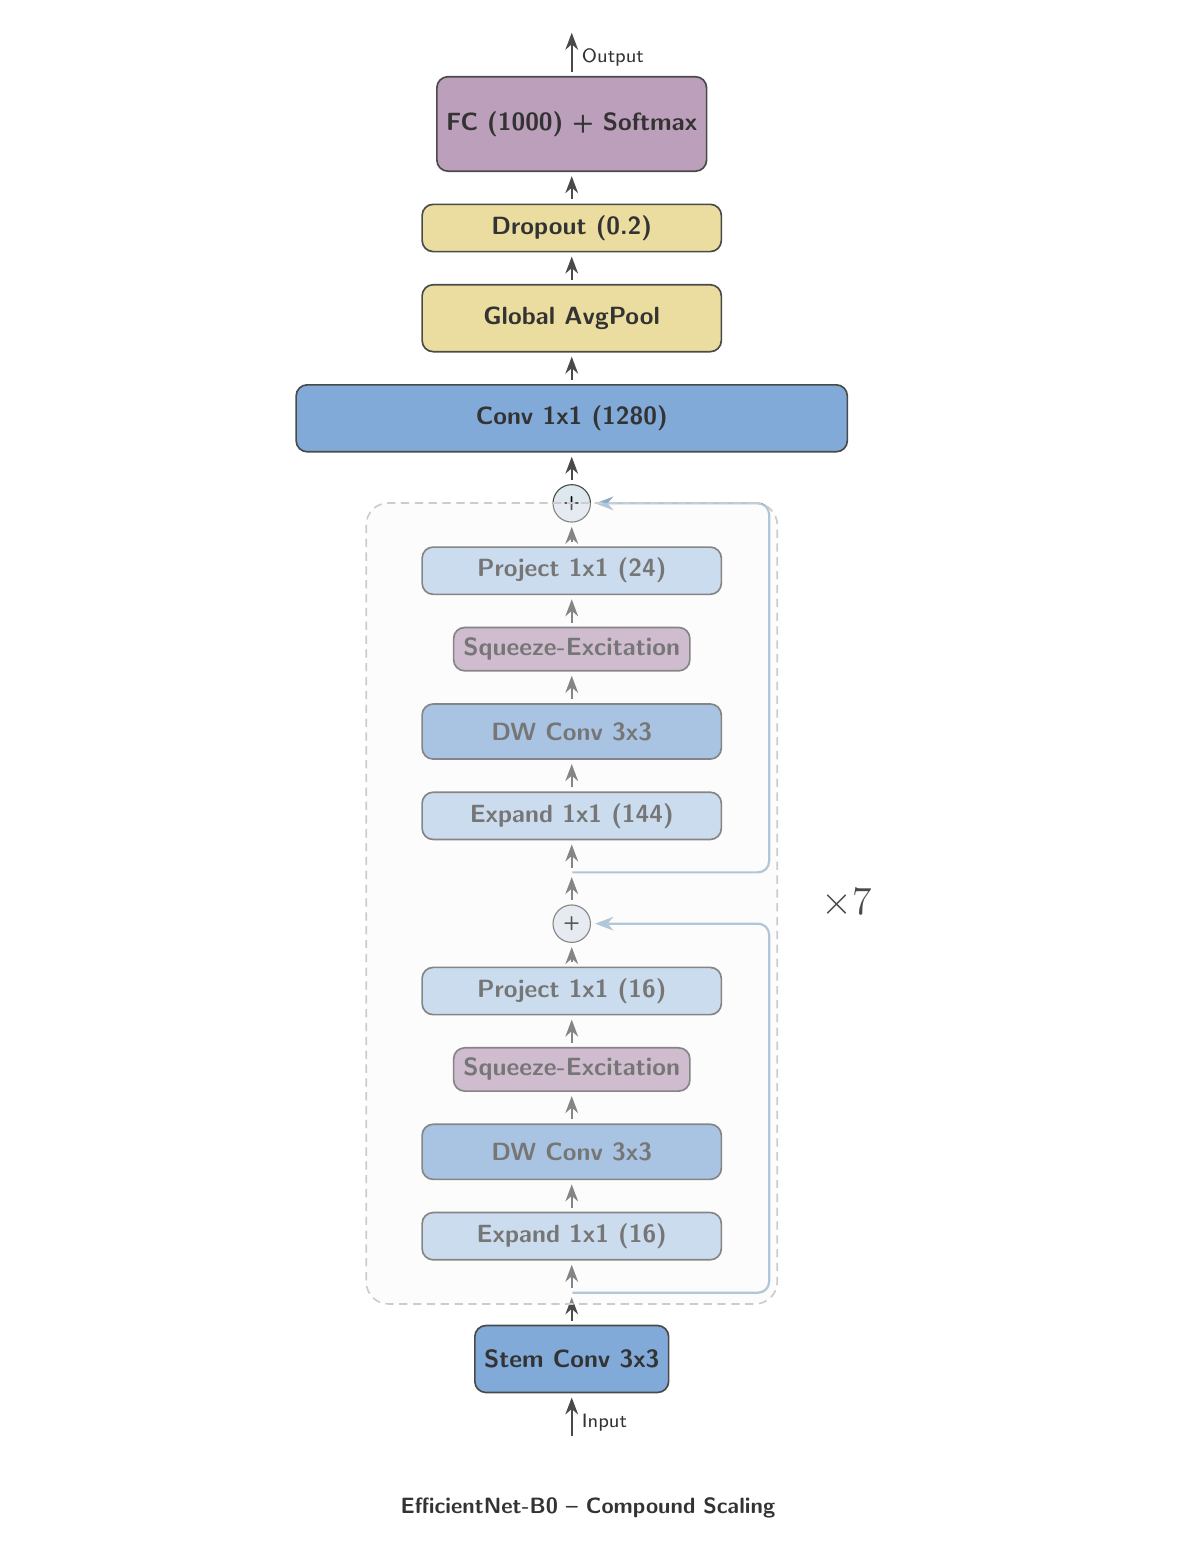
\begin{tikzpicture}[
    >=Stealth,
    every node/.style={font=\sffamily},
    block/.style={draw=clrborder, rounded corners=4pt, minimum width=3.8cm,
                  minimum height=0.85cm, font=\sffamily\small\bfseries,
                  text=clrtext, line width=0.6pt},
    arrow/.style={->, thick, color=clrborder, line width=0.7pt, shorten >=1.5pt, shorten <=1.5pt},
    skiparrow/.style={->, thick, color=clrresidual, line width=0.8pt, rounded corners=4pt, shorten >=1.5pt},
    label/.style={font=\sffamily\scriptsize, text=clrtext},
    subtitle/.style={font=\sffamily\footnotesize, text=clrtext},
]
\node[block, fill=clrattention!85, minimum width=1.5cm, minimum height=0.85cm, text=clrtext] (n_1) at (0,0) {Stem Conv 3x3};
\node[inner sep=0, minimum size=0, above=0.4cm of n_1] (res_entry_2) {};
\node[block, fill=clrattention_alt!85, minimum width=3.8cm, minimum height=0.6cm, text=clrtext, above=0.4cm of res_entry_2] (n_3) {Expand 1x1 (16)};
\node[block, fill=clrattention!85, minimum width=3.8cm, minimum height=0.7cm, text=clrtext, above=0.4cm of n_3] (n_4) {DW Conv 3x3};
\node[block, fill=clroutput!85, minimum width=3.0cm, minimum height=0.55cm, text=clrtext, above=0.4cm of n_4] (n_5) {Squeeze-Excitation};
\node[block, fill=clrattention_alt!85, minimum width=3.8cm, minimum height=0.6cm, text=clrtext, above=0.4cm of n_5] (n_6) {Project 1x1 (16)};
\node[circle, draw=clrborder, fill=clrresidual!30, inner sep=2pt, font=\sffamily\scriptsize\bfseries, above=0.3cm of n_6] (add_7) {+};
\node[inner sep=0, minimum size=0, above=0.4cm of add_7] (res_entry_8) {};
\node[block, fill=clrattention_alt!85, minimum width=3.8cm, minimum height=0.6cm, text=clrtext, above=0.4cm of res_entry_8] (n_9) {Expand 1x1 (144)};
\node[block, fill=clrattention!85, minimum width=3.8cm, minimum height=0.7cm, text=clrtext, above=0.4cm of n_9] (n_10) {DW Conv 3x3};
\node[block, fill=clroutput!85, minimum width=3.0cm, minimum height=0.55cm, text=clrtext, above=0.4cm of n_10] (n_11) {Squeeze-Excitation};
\node[block, fill=clrattention_alt!85, minimum width=3.8cm, minimum height=0.6cm, text=clrtext, above=0.4cm of n_11] (n_12) {Project 1x1 (24)};
\node[circle, draw=clrborder, fill=clrresidual!30, inner sep=2pt, font=\sffamily\scriptsize\bfseries, above=0.3cm of n_12] (add_13) {+};
\node[block, fill=clrattention!85, minimum width=7.0cm, minimum height=0.85cm, text=clrtext, above=0.4cm of add_13] (n_14) {Conv 1x1 (1280)};
\node[block, fill=clrnorm!85, minimum width=3.8cm, minimum height=0.85cm, text=clrtext, above=0.4cm of n_14] (n_15) {Global AvgPool};
\node[block, fill=clrnorm!85, minimum width=3.8cm, minimum height=0.6cm, text=clrtext, above=0.4cm of n_15] (n_16) {Dropout (0.2)};
\node[block, fill=clroutput!85, minimum width=2.0cm, minimum height=1.2cm, text=clrtext, above=0.4cm of n_16] (n_17) {FC (1000) + Softmax};
\draw[arrow] (n_3.north) -- (n_4.south);
\draw[arrow] (n_4.north) -- (n_5.south);
\draw[arrow] (n_5.north) -- (n_6.south);
\draw[arrow] (res_entry_2.north) -- (n_3.south);
\draw[arrow] (n_6.north) -- (add_7.south);
\draw[skiparrow] (res_entry_2.east) -- ++(2.5,0) |- (add_7.east);
\draw[arrow] (n_1.north) -- (res_entry_2.south);
\draw[arrow] (n_9.north) -- (n_10.south);
\draw[arrow] (n_10.north) -- (n_11.south);
\draw[arrow] (n_11.north) -- (n_12.south);
\draw[arrow] (res_entry_8.north) -- (n_9.south);
\draw[arrow] (n_12.north) -- (add_13.south);
\draw[skiparrow] (res_entry_8.east) -- ++(2.5,0) |- (add_13.east);
\draw[arrow] (add_7.north) -- (res_entry_8.south);
\draw[arrow] (add_13.north) -- (n_14.south);
\draw[arrow] (n_14.north) -- (n_15.south);
\draw[arrow] (n_15.north) -- (n_16.south);
\draw[arrow] (n_16.north) -- (n_17.south);
\draw[arrow] ([yshift=-0.6cm]n_1.south) -- node[right, yshift=-2pt, font=\sffamily\scriptsize, text=clrtext] {Input} (n_1.south);
\draw[arrow] (n_17.north) -- node[right, yshift=-2pt, font=\sffamily\scriptsize, text=clrtext] {Output} ([yshift=0.6cm]n_17.north);
\node[draw=clrgroup_frame!60, rounded corners=8pt, densely dashed, line width=0.6pt, fill=clrgroup_fill, fill opacity=0.35, inner ysep=0.55cm, inner xsep=0.7cm, fit=(n_3) (n_4) (n_5) (n_6) (n_9) (n_10) (n_11) (n_12)] (g_0) {};
\node[right=12pt of g_0.east, anchor=west, font=\sffamily\Large\bfseries, text=clrborder] (g_0_badge) {$\times7$};
\node[below=0.6cm of current bounding box.south, subtitle, text width=14cm, align=center] {\textbf{EfficientNet-B0 -- Compound Scaling}};
\end{tikzpicture}
\end{document}
